\documentclass{article}
\usepackage{graphicx} 
\title{Requirements and Design Documentation}
\author{devs101}

\begin{document}
\tableofcontents
\newpage

\section{Functional Requirements}
The Editor must be able to do the following:
\begin{itemize}
\item Add a new node to the tree.
\item Move an existing node around in the tree view.
\item Delete an existing node from the tree.
\item Copy a node and all its properties.
\item Paste a copied node to the tree view.
\item Edit the following settings of a node:
 \begin{itemize}
  \item	Name
  \item ID
  \item Description
  \item Visible
  \item Enabled
  \item Max
  \item Cost
 \end{itemize}
\item Links between nodes must be automatically created, but links can also be manually set and changed in the editor.
\item Save and Load the state of the tree at any point in time. Save data must be stored in a JSON format.
\item Undo and Redo any actions or changes performed on the tree at any point in time. Must be able to undo as many times as actions where performed, undo until original tree state is reached.
\item Multi selection of nodes. Must be able to select multiple nodes at once and perform all node operations (Move, Copy, Paste, Delete, Edit, etc.) to all selected nodes at once.
\item Automatically produce a layout of the current nodes.
\item Zoom in and out of the tree view.
\item The user must also be able to create custom global variables that will be used in the tree structure.
\item The custom variables must be usable in the node settings.
\end{itemize}

Testing must be performed on the skill tree.

\begin{itemize}
\item Users should specify global variable values and amount of skill points available
\item User should be able to buy skills with skill points
\item User should be able to reset skill points
\item Must create a JavaScript file that web developers can use to import, display and use a skill tree on their own webpage.
\begin{itemize}
\item Allow the developer to give a skill tree json file that can set global parameters and set initial selected skills.
\item Allow the developer to query what skills have been selected.
\item Allow the developer to trigger their own functions when skills are selected.
\item All these functionality should be demonstrated with jsFiddle.
\end{itemize}
\item Allow users to edit how the nodes, links and background looks.
\end{itemize}

\section{Domain Model}

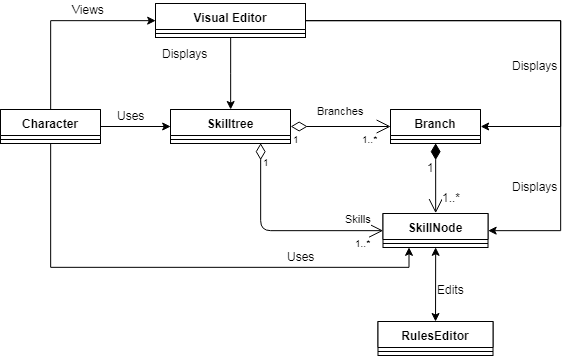
\includegraphics{TriiDomainModel}

\section{Architectural Design and Structure}

The Trii system is based on the Client-Server architecture style. This is because the website is the server that provides the service of the skill tree software to several clients that connect to the server. The clients can connect from anywhere to the server via a http protocol and use the software from their own work station.

\end{document}